\documentclass[1p]{elsarticle_modified}
%\bibliographystyle{elsarticle-num}

%\usepackage[colorlinks]{hyperref}
%\usepackage{abbrmath_seonhwa} %\Abb, \Ascr, \Acal ,\Abf, \Afrak
\usepackage{amsfonts}
\usepackage{amssymb}
\usepackage{amsmath}
\usepackage{amsthm}
\usepackage{scalefnt}
\usepackage{amsbsy}
\usepackage{kotex}
\usepackage{caption}
\usepackage{subfig}
\usepackage{color}
\usepackage{graphicx}
\usepackage{xcolor} %% white, black, red, green, blue, cyan, magenta, yellow
\usepackage{float}
\usepackage{setspace}
\usepackage{hyperref}

\usepackage{tikz}
\usetikzlibrary{arrows}

\usepackage{multirow}
\usepackage{array} % fixed length table
\usepackage{hhline}

%%%%%%%%%%%%%%%%%%%%%
\makeatletter
\renewcommand*\env@matrix[1][\arraystretch]{%
	\edef\arraystretch{#1}%
	\hskip -\arraycolsep
	\let\@ifnextchar\new@ifnextchar
	\array{*\c@MaxMatrixCols c}}
\makeatother %https://tex.stackexchange.com/questions/14071/how-can-i-increase-the-line-spacing-in-a-matrix
%%%%%%%%%%%%%%%

\usepackage[normalem]{ulem}

\newcommand{\msout}[1]{\ifmmode\text{\sout{\ensuremath{#1}}}\else\sout{#1}\fi}
%SOURCE: \msout is \stkout macro in https://tex.stackexchange.com/questions/20609/strikeout-in-math-mode

\newcommand{\cancel}[1]{
	\ifmmode
	{\color{red}\msout{#1}}
	\else
	{\color{red}\sout{#1}}
	\fi
}

\newcommand{\add}[1]{
	{\color{blue}\uwave{#1}}
}

\newcommand{\replace}[2]{
	\ifmmode
	{\color{red}\msout{#1}}{\color{blue}\uwave{#2}}
	\else
	{\color{red}\sout{#1}}{\color{blue}\uwave{#2}}
	\fi
}

\newcommand{\Sol}{\mathcal{S}} %segment
\newcommand{\D}{D} %diagram
\newcommand{\A}{\mathcal{A}} %arc


%%%%%%%%%%%%%%%%%%%%%%%%%%%%%5 test

\def\sl{\operatorname{\textup{SL}}(2,\Cbb)}
\def\psl{\operatorname{\textup{PSL}}(2,\Cbb)}
\def\quan{\mkern 1mu \triangleright \mkern 1mu}

\theoremstyle{definition}
\newtheorem{thm}{Theorem}[section]
\newtheorem{prop}[thm]{Proposition}
\newtheorem{lem}[thm]{Lemma}
\newtheorem{ques}[thm]{Question}
\newtheorem{cor}[thm]{Corollary}
\newtheorem{defn}[thm]{Definition}
\newtheorem{exam}[thm]{Example}
\newtheorem{rmk}[thm]{Remark}
\newtheorem{alg}[thm]{Algorithm}

\newcommand{\I}{\sqrt{-1}}
\begin{document}

%\begin{frontmatter}
%
%\title{Boundary parabolic representations of knots up to 8 crossings}
%
%%% Group authors per affiliation:
%\author{Yunhi Cho} 
%\address{Department of Mathematics, University of Seoul, Seoul, Korea}
%\ead{yhcho@uos.ac.kr}
%
%
%\author{Seonhwa Kim} %\fnref{s_kim}}
%\address{Center for Geometry and Physics, Institute for Basic Science, Pohang, 37673, Korea}
%\ead{ryeona17@ibs.re.kr}
%
%\author{Hyuk Kim}
%\address{Department of Mathematical Sciences, Seoul National University, Seoul 08826, Korea}
%\ead{hyukkim@snu.ac.kr}
%
%\author{Seokbeom Yoon}
%\address{Department of Mathematical Sciences, Seoul National University, Seoul, 08826,  Korea}
%\ead{sbyoon15@snu.ac.kr}
%
%\begin{abstract}
%We find all boundary parabolic representation of knots up to 8 crossings.
%
%\end{abstract}
%\begin{keyword}
%    \MSC[2010] 57M25 
%\end{keyword}
%
%\end{frontmatter}

%\linenumbers
%\tableofcontents
%
\newcommand\colored[1]{\textcolor{white}{\rule[-0.35ex]{0.8em}{1.4ex}}\kern-0.8em\color{red} #1}%
%\newcommand\colored[1]{\textcolor{white}{ #1}\kern-2.17ex	\textcolor{white}{ #1}\kern-1.81ex	\textcolor{white}{ #1}\kern-2.15ex\color{red}#1	}

{\Large $\underline{12n_{0391}~(K12n_{0391})}$}

\setlength{\tabcolsep}{10pt}
\renewcommand{\arraystretch}{1.6}
\vspace{1cm}\begin{tabular}{m{100pt}>{\centering\arraybackslash}m{274pt}}
\multirow{5}{120pt}{
	\centering
	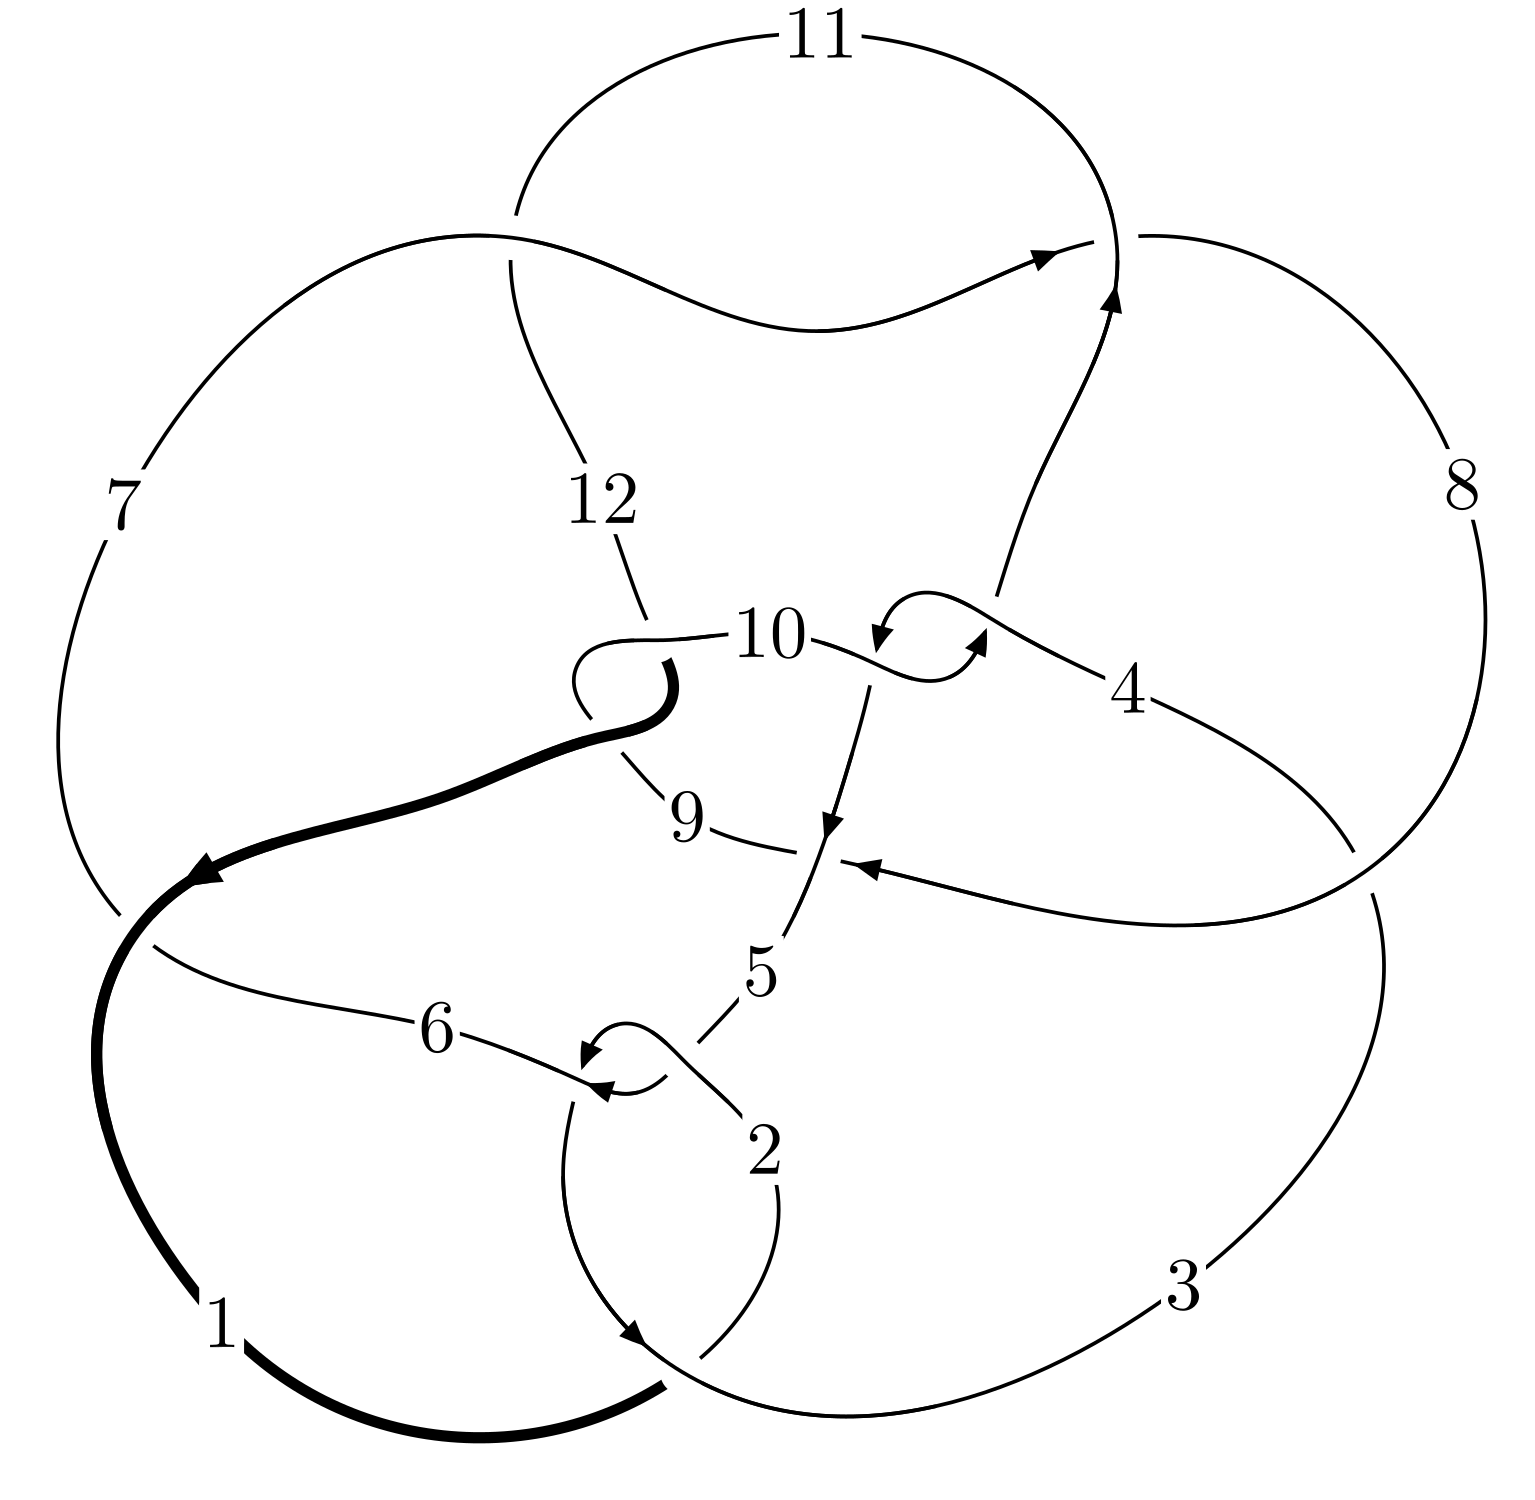
\includegraphics[width=112pt]{../../../GIT/diagram.site/Diagrams/png/2480_12n_0391.png}\\
\ \ \ A knot diagram\footnotemark}&
\allowdisplaybreaks
\textbf{Linearized knot diagam} \\
\cline{2-2}
 &
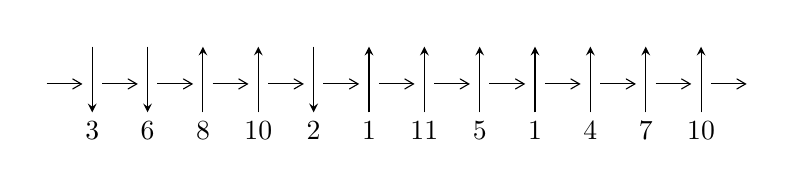
\begin{tikzpicture}[x=20pt, y=17pt]
	% nodes
	\node (C0) at (0, 0) {};
	\node (C1) at (1, 0) {};
	\node (C1U) at (1, +1) {};
	\node (C1D) at (1, -1) {3};

	\node (C2) at (2, 0) {};
	\node (C2U) at (2, +1) {};
	\node (C2D) at (2, -1) {6};

	\node (C3) at (3, 0) {};
	\node (C3U) at (3, +1) {};
	\node (C3D) at (3, -1) {8};

	\node (C4) at (4, 0) {};
	\node (C4U) at (4, +1) {};
	\node (C4D) at (4, -1) {10};

	\node (C5) at (5, 0) {};
	\node (C5U) at (5, +1) {};
	\node (C5D) at (5, -1) {2};

	\node (C6) at (6, 0) {};
	\node (C6U) at (6, +1) {};
	\node (C6D) at (6, -1) {1};

	\node (C7) at (7, 0) {};
	\node (C7U) at (7, +1) {};
	\node (C7D) at (7, -1) {11};

	\node (C8) at (8, 0) {};
	\node (C8U) at (8, +1) {};
	\node (C8D) at (8, -1) {5};

	\node (C9) at (9, 0) {};
	\node (C9U) at (9, +1) {};
	\node (C9D) at (9, -1) {1};

	\node (C10) at (10, 0) {};
	\node (C10U) at (10, +1) {};
	\node (C10D) at (10, -1) {4};

	\node (C11) at (11, 0) {};
	\node (C11U) at (11, +1) {};
	\node (C11D) at (11, -1) {7};

	\node (C12) at (12, 0) {};
	\node (C12U) at (12, +1) {};
	\node (C12D) at (12, -1) {10};
	\node (C13) at (13, 0) {};

	% arrows
	\draw[->,>={angle 60}]
	(C0) edge (C1) (C1) edge (C2) (C2) edge (C3) (C3) edge (C4) (C4) edge (C5) (C5) edge (C6) (C6) edge (C7) (C7) edge (C8) (C8) edge (C9) (C9) edge (C10) (C10) edge (C11) (C11) edge (C12) (C12) edge (C13) ;	\draw[->,>=stealth]
	(C1U) edge (C1D) (C2U) edge (C2D) (C3D) edge (C3U) (C4D) edge (C4U) (C5U) edge (C5D) (C6D) edge (C6U) (C7D) edge (C7U) (C8D) edge (C8U) (C9D) edge (C9U) (C10D) edge (C10U) (C11D) edge (C11U) (C12D) edge (C12U) ;
	\end{tikzpicture} \\
\hhline{~~} \\& 
\textbf{Solving Sequence} \\ \cline{2-2} 
 &
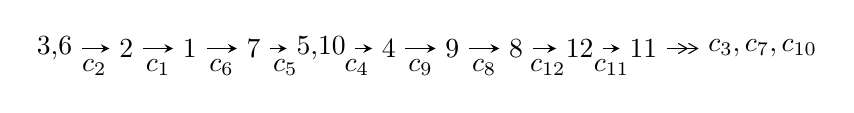
\begin{tikzpicture}[x=23pt, y=7pt]
	% node
	\node (A0) at (-1/8, 0) {3,6};
	\node (A1) at (1, 0) {2};
	\node (A2) at (2, 0) {1};
	\node (A3) at (3, 0) {7};
	\node (A4) at (65/16, 0) {5,10};
	\node (A5) at (41/8, 0) {4};
	\node (A6) at (49/8, 0) {9};
	\node (A7) at (57/8, 0) {8};
	\node (A8) at (65/8, 0) {12};
	\node (A9) at (73/8, 0) {11};
	\node (C1) at (1/2, -1) {$c_{2}$};
	\node (C2) at (3/2, -1) {$c_{1}$};
	\node (C3) at (5/2, -1) {$c_{6}$};
	\node (C4) at (7/2, -1) {$c_{5}$};
	\node (C5) at (37/8, -1) {$c_{4}$};
	\node (C6) at (45/8, -1) {$c_{9}$};
	\node (C7) at (53/8, -1) {$c_{8}$};
	\node (C8) at (61/8, -1) {$c_{12}$};
	\node (C9) at (69/8, -1) {$c_{11}$};
	\node (A10) at (11, 0) {$c_{3},c_{7},c_{10}$};

	% edge
	\draw[->,>=stealth]	
	(A0) edge (A1) (A1) edge (A2) (A2) edge (A3) (A3) edge (A4) (A4) edge (A5) (A5) edge (A6) (A6) edge (A7) (A7) edge (A8) (A8) edge (A9) ;
	\draw[->>,>={angle 60}]	
	(A9) edge (A10);
\end{tikzpicture} \\ 

\end{tabular} \\

\footnotetext{
The image of knot diagram is generated by the software ``\textbf{Draw programme}" developed by Andrew Bartholomew(\url{http://www.layer8.co.uk/maths/draw/index.htm\#Running-draw}), where we modified some parts for our purpose(\url{https://github.com/CATsTAILs/LinksPainter}).
}\phantom \\ \newline 
\centering \textbf{Ideals for irreducible components\footnotemark of $X_{\text{par}}$} 
 
\begin{align*}
I^u_{1}&=\langle 
3 u^{32}-10 u^{31}+\cdots+2 b+4,\;5 u^{32}-31 u^{31}+\cdots+2 a-35,\;u^{33}-6 u^{32}+\cdots-10 u+4\rangle \\
I^u_{2}&=\langle 
-47109570 u^{10} a^3-95144015 u^{10} a^2+\cdots-183653747 a-331708329,\\
\phantom{I^u_{2}}&\phantom{= \langle  }-2 u^{10} a^3- u^{10} a^2+\cdots+3 a^2-2 a,\;u^{11}+u^{10}-2 u^9-3 u^8+2 u^7+4 u^6-3 u^4- u^3+u^2-1\rangle \\
I^u_{3}&=\langle 
- u^{19}- u^{18}+\cdots+b-1,\\
\phantom{I^u_{3}}&\phantom{= \langle  }u^{16}+u^{15}-4 u^{14}-5 u^{13}+7 u^{12}+11 u^{11}-4 u^{10}-12 u^9-3 u^8+5 u^7+5 u^6+2 u^5-3 u^3-3 u^2+a+u+1,\\
\phantom{I^u_{3}}&\phantom{= \langle  }u^{20}+u^{19}+\cdots+u+1\rangle \\
\\
\end{align*}
\raggedright * 3 irreducible components of $\dim_{\mathbb{C}}=0$, with total 97 representations.\\
\footnotetext{All coefficients of polynomials are rational numbers. But the coefficients are sometimes approximated in decimal forms when there is not enough margin.}
\newpage
\renewcommand{\arraystretch}{1}
\centering \section*{I. $I^u_{1}= \langle 3 u^{32}-10 u^{31}+\cdots+2 b+4,\;5 u^{32}-31 u^{31}+\cdots+2 a-35,\;u^{33}-6 u^{32}+\cdots-10 u+4 \rangle$}
\flushleft \textbf{(i) Arc colorings}\\
\begin{tabular}{m{7pt} m{180pt} m{7pt} m{180pt} }
\flushright $a_{3}=$&$\begin{pmatrix}1\\0\end{pmatrix}$ \\
\flushright $a_{6}=$&$\begin{pmatrix}0\\u\end{pmatrix}$ \\
\flushright $a_{2}=$&$\begin{pmatrix}1\\- u^2\end{pmatrix}$ \\
\flushright $a_{1}=$&$\begin{pmatrix}- u^2+1\\- u^2\end{pmatrix}$ \\
\flushright $a_{7}=$&$\begin{pmatrix}u^5-2 u^3+u\\u^5- u^3+u\end{pmatrix}$ \\
\flushright $a_{5}=$&$\begin{pmatrix}u\\- u^3+u\end{pmatrix}$ \\
\flushright $a_{10}=$&$\begin{pmatrix}-\frac{5}{2} u^{32}+\frac{31}{2} u^{31}+\cdots-27 u+\frac{35}{2}\\-\frac{3}{2} u^{32}+5 u^{31}+\cdots-\frac{1}{2} u-2\end{pmatrix}$ \\
\flushright $a_{4}=$&$\begin{pmatrix}-\frac{1}{4} u^{32}+3 u^{31}+\cdots-\frac{21}{4} u+4\\-\frac{5}{2} u^{32}+13 u^{31}+\cdots-\frac{29}{2} u+7\end{pmatrix}$ \\
\flushright $a_{9}=$&$\begin{pmatrix}-5 u^{32}+\frac{43}{2} u^{31}+\cdots-\frac{39}{2} u+\frac{3}{2}\\\frac{9}{2} u^{32}-31 u^{31}+\cdots+\frac{111}{2} u-38\end{pmatrix}$ \\
\flushright $a_{8}=$&$\begin{pmatrix}- u^{32}+\frac{5}{2} u^{31}+\cdots-\frac{5}{2} u-\frac{9}{2}\\\frac{13}{2} u^{32}-32 u^{31}+\cdots+\frac{77}{2} u-24\end{pmatrix}$ \\
\flushright $a_{12}=$&$\begin{pmatrix}\frac{3}{4} u^{32}-6 u^{31}+\cdots+\frac{39}{4} u-11\\\frac{13}{2} u^{32}-32 u^{31}+\cdots+\frac{81}{2} u-25\end{pmatrix}$ \\
\flushright $a_{11}=$&$\begin{pmatrix}-\frac{13}{4} u^{32}+18 u^{31}+\cdots-\frac{121}{4} u+19\\\frac{3}{2} u^{32}-8 u^{31}+\cdots+\frac{21}{2} u-7\end{pmatrix}$\\&\end{tabular}
\flushleft \textbf{(ii) Obstruction class $= -1$}\\~\\
\flushleft \textbf{(iii) Cusp Shapes $= 19 u^{32}-93 u^{31}+87 u^{30}+399 u^{29}-1093 u^{28}+124 u^{27}+3263 u^{26}-4355 u^{25}-2560 u^{24}+11701 u^{23}-7466 u^{22}-11755 u^{21}+22346 u^{20}-4792 u^{19}-23413 u^{18}+26009 u^{17}+2484 u^{16}-27634 u^{15}+20515 u^{14}+6968 u^{13}-21858 u^{12}+11815 u^{11}+6157 u^{10}-12060 u^9+4832 u^8+3318 u^7-4487 u^6+1156 u^5+1213 u^4-1111 u^3+245 u^2+110 u-54$}\\~\\
\newpage\renewcommand{\arraystretch}{1}
\flushleft \textbf{(iv) u-Polynomials at the component}\newline \\
\begin{tabular}{m{50pt}|m{274pt}}
Crossings & \hspace{64pt}u-Polynomials at each crossing \\
\hline $$\begin{aligned}c_{1}\end{aligned}$$&$\begin{aligned}
&u^{33}+16 u^{32}+\cdots+172 u+16
\end{aligned}$\\
\hline $$\begin{aligned}c_{2},c_{5}\end{aligned}$$&$\begin{aligned}
&u^{33}+6 u^{32}+\cdots-10 u-4
\end{aligned}$\\
\hline $$\begin{aligned}c_{3},c_{4},c_{10}\end{aligned}$$&$\begin{aligned}
&u^{33}+9 u^{31}+\cdots+2 u-1
\end{aligned}$\\
\hline $$\begin{aligned}c_{6}\end{aligned}$$&$\begin{aligned}
&u^{33}+18 u^{32}+\cdots-1198 u-188
\end{aligned}$\\
\hline $$\begin{aligned}c_{7},c_{11}\end{aligned}$$&$\begin{aligned}
&u^{33}-24 u^{32}+\cdots+26624 u-2048
\end{aligned}$\\
\hline $$\begin{aligned}c_{8}\end{aligned}$$&$\begin{aligned}
&u^{33}- u^{32}+\cdots+106 u-23
\end{aligned}$\\
\hline $$\begin{aligned}c_{9},c_{12}\end{aligned}$$&$\begin{aligned}
&u^{33}+2 u^{32}+\cdots-16 u-1
\end{aligned}$\\
\hline
\end{tabular}\\~\\
\newpage\renewcommand{\arraystretch}{1}
\flushleft \textbf{(v) Riley Polynomials at the component}\newline \\
\begin{tabular}{m{50pt}|m{274pt}}
Crossings & \hspace{64pt}Riley Polynomials at each crossing \\
\hline $$\begin{aligned}c_{1}\end{aligned}$$&$\begin{aligned}
&y^{33}+4 y^{32}+\cdots+9456 y-256
\end{aligned}$\\
\hline $$\begin{aligned}c_{2},c_{5}\end{aligned}$$&$\begin{aligned}
&y^{33}-16 y^{32}+\cdots+172 y-16
\end{aligned}$\\
\hline $$\begin{aligned}c_{3},c_{4},c_{10}\end{aligned}$$&$\begin{aligned}
&y^{33}+18 y^{32}+\cdots-4 y-1
\end{aligned}$\\
\hline $$\begin{aligned}c_{6}\end{aligned}$$&$\begin{aligned}
&y^{33}+8 y^{32}+\cdots+252684 y-35344
\end{aligned}$\\
\hline $$\begin{aligned}c_{7},c_{11}\end{aligned}$$&$\begin{aligned}
&y^{33}+12 y^{32}+\cdots+2097152 y-4194304
\end{aligned}$\\
\hline $$\begin{aligned}c_{8}\end{aligned}$$&$\begin{aligned}
&y^{33}-31 y^{32}+\cdots+16020 y-529
\end{aligned}$\\
\hline $$\begin{aligned}c_{9},c_{12}\end{aligned}$$&$\begin{aligned}
&y^{33}-42 y^{32}+\cdots+54 y-1
\end{aligned}$\\
\hline
\end{tabular}\\~\\
\newpage\flushleft \textbf{(vi) Complex Volumes and Cusp Shapes}
$$\begin{array}{c|c|c}  
\text{Solutions to }I^u_{1}& \I (\text{vol} + \sqrt{-1}CS) & \text{Cusp shape}\\
 \hline 
\begin{aligned}
u &= \phantom{-}0.615043 + 0.794458 I \\
a &= -0.931151 + 0.481633 I \\
b &= -1.158050 + 0.155662 I\end{aligned}
 & \phantom{-}2.15328 - 7.47057 I & \phantom{-}6.28978 + 6.05240 I \\ \hline\begin{aligned}
u &= \phantom{-}0.615043 - 0.794458 I \\
a &= -0.931151 - 0.481633 I \\
b &= -1.158050 - 0.155662 I\end{aligned}
 & \phantom{-}2.15328 + 7.47057 I & \phantom{-}6.28978 - 6.05240 I \\ \hline\begin{aligned}
u &= \phantom{-}0.934351 + 0.256317 I \\
a &= \phantom{-}0.138141 - 0.042111 I \\
b &= -0.307888 - 0.461843 I\end{aligned}
 & -1.58520 - 0.97498 I & -1.65033 + 1.59039 I \\ \hline\begin{aligned}
u &= \phantom{-}0.934351 - 0.256317 I \\
a &= \phantom{-}0.138141 + 0.042111 I \\
b &= -0.307888 + 0.461843 I\end{aligned}
 & -1.58520 + 0.97498 I & -1.65033 - 1.59039 I \\ \hline\begin{aligned}
u &= \phantom{-}0.402264 + 0.852871 I \\
a &= -1.58643 - 1.26589 I \\
b &= -1.72042 - 0.99064 I\end{aligned}
 & \phantom{-}0.89438 + 10.98450 I & \phantom{-}5.23661 - 5.54944 I \\ \hline\begin{aligned}
u &= \phantom{-}0.402264 - 0.852871 I \\
a &= -1.58643 + 1.26589 I \\
b &= -1.72042 + 0.99064 I\end{aligned}
 & \phantom{-}0.89438 - 10.98450 I & \phantom{-}5.23661 + 5.54944 I \\ \hline\begin{aligned}
u &= -0.927183 + 0.525541 I \\
a &= -1.014440 + 0.779993 I \\
b &= -0.742899 - 0.107800 I\end{aligned}
 & \phantom{-}0.18348 + 3.87388 I & \phantom{-}6.31776 - 7.47791 I \\ \hline\begin{aligned}
u &= -0.927183 - 0.525541 I \\
a &= -1.014440 - 0.779993 I \\
b &= -0.742899 + 0.107800 I\end{aligned}
 & \phantom{-}0.18348 - 3.87388 I & \phantom{-}6.31776 + 7.47791 I \\ \hline\begin{aligned}
u &= \phantom{-}0.582669 + 0.708437 I \\
a &= \phantom{-}0.741361 + 0.151629 I \\
b &= \phantom{-}1.178060 + 0.561251 I\end{aligned}
 & \phantom{-}4.85669 - 0.62382 I & \phantom{-}7.67399 + 3.72585 I \\ \hline\begin{aligned}
u &= \phantom{-}0.582669 - 0.708437 I \\
a &= \phantom{-}0.741361 - 0.151629 I \\
b &= \phantom{-}1.178060 - 0.561251 I\end{aligned}
 & \phantom{-}4.85669 + 0.62382 I & \phantom{-}7.67399 - 3.72585 I\\
 \hline 
 \end{array}$$\newpage$$\begin{array}{c|c|c}  
\text{Solutions to }I^u_{1}& \I (\text{vol} + \sqrt{-1}CS) & \text{Cusp shape}\\
 \hline 
\begin{aligned}
u &= \phantom{-}0.355906 + 0.802794 I \\
a &= \phantom{-}1.57216 + 0.88862 I \\
b &= \phantom{-}1.72277 + 0.45864 I\end{aligned}
 & \phantom{-}3.58955 + 3.24533 I & \phantom{-}5.20458 - 3.30279 I \\ \hline\begin{aligned}
u &= \phantom{-}0.355906 - 0.802794 I \\
a &= \phantom{-}1.57216 - 0.88862 I \\
b &= \phantom{-}1.72277 - 0.45864 I\end{aligned}
 & \phantom{-}3.58955 - 3.24533 I & \phantom{-}5.20458 + 3.30279 I \\ \hline\begin{aligned}
u &= \phantom{-}0.050477 + 0.847272 I \\
a &= -1.032160 - 0.468103 I \\
b &= -0.777802 - 0.129336 I\end{aligned}
 & -5.00986 - 1.85205 I & \phantom{-}6.76082 + 4.03630 I \\ \hline\begin{aligned}
u &= \phantom{-}0.050477 - 0.847272 I \\
a &= -1.032160 + 0.468103 I \\
b &= -0.777802 + 0.129336 I\end{aligned}
 & -5.00986 + 1.85205 I & \phantom{-}6.76082 - 4.03630 I \\ \hline\begin{aligned}
u &= \phantom{-}1.010310 + 0.608408 I \\
a &= -0.98297 - 1.05108 I \\
b &= -0.855242 + 0.984190 I\end{aligned}
 & \phantom{-}3.58006 - 4.43418 I & \phantom{-}6.35662 + 2.15933 I \\ \hline\begin{aligned}
u &= \phantom{-}1.010310 - 0.608408 I \\
a &= -0.98297 + 1.05108 I \\
b &= -0.855242 - 0.984190 I\end{aligned}
 & \phantom{-}3.58006 + 4.43418 I & \phantom{-}6.35662 - 2.15933 I \\ \hline\begin{aligned}
u &= -1.159600 + 0.228047 I \\
a &= \phantom{-}0.786672 + 0.851083 I \\
b &= -1.034420 + 0.855065 I\end{aligned}
 & -1.231110 - 0.428619 I & -1.25867 + 1.75566 I \\ \hline\begin{aligned}
u &= -1.159600 - 0.228047 I \\
a &= \phantom{-}0.786672 - 0.851083 I \\
b &= -1.034420 - 0.855065 I\end{aligned}
 & -1.231110 + 0.428619 I & -1.25867 - 1.75566 I \\ \hline\begin{aligned}
u &= -0.717593 + 0.390417 I \\
a &= \phantom{-}1.47547 - 0.34302 I \\
b &= \phantom{-}0.464162 + 0.242439 I\end{aligned}
 & \phantom{-}0.934933 + 0.153832 I & \phantom{-}10.03665 - 0.30542 I \\ \hline\begin{aligned}
u &= -0.717593 - 0.390417 I \\
a &= \phantom{-}1.47547 + 0.34302 I \\
b &= \phantom{-}0.464162 - 0.242439 I\end{aligned}
 & \phantom{-}0.934933 - 0.153832 I & \phantom{-}10.03665 + 0.30542 I\\
 \hline 
 \end{array}$$\newpage$$\begin{array}{c|c|c}  
\text{Solutions to }I^u_{1}& \I (\text{vol} + \sqrt{-1}CS) & \text{Cusp shape}\\
 \hline 
\begin{aligned}
u &= \phantom{-}0.998884 + 0.676093 I \\
a &= \phantom{-}0.251045 + 1.284470 I \\
b &= \phantom{-}0.779513 - 0.138727 I\end{aligned}
 & \phantom{-}1.00418 + 1.96266 I & \phantom{-}5.00130 - 1.18904 I \\ \hline\begin{aligned}
u &= \phantom{-}0.998884 - 0.676093 I \\
a &= \phantom{-}0.251045 - 1.284470 I \\
b &= \phantom{-}0.779513 + 0.138727 I\end{aligned}
 & \phantom{-}1.00418 - 1.96266 I & \phantom{-}5.00130 + 1.18904 I \\ \hline\begin{aligned}
u &= -1.206650 + 0.128661 I \\
a &= -0.777551 - 0.265371 I \\
b &= \phantom{-}1.07673 - 1.12681 I\end{aligned}
 & -4.62253 - 8.29061 I & -0.38123 + 5.10542 I \\ \hline\begin{aligned}
u &= -1.206650 - 0.128661 I \\
a &= -0.777551 + 0.265371 I \\
b &= \phantom{-}1.07673 + 1.12681 I\end{aligned}
 & -4.62253 + 8.29061 I & -0.38123 - 5.10542 I \\ \hline\begin{aligned}
u &= \phantom{-}1.137250 + 0.591003 I \\
a &= -1.26745 - 1.33966 I \\
b &= -1.96175 + 0.78277 I\end{aligned}
 & \phantom{-}1.26915 - 8.46714 I & \phantom{-}2.03049 + 6.90183 I \\ \hline\begin{aligned}
u &= \phantom{-}1.137250 - 0.591003 I \\
a &= -1.26745 + 1.33966 I \\
b &= -1.96175 - 0.78277 I\end{aligned}
 & \phantom{-}1.26915 + 8.46714 I & \phantom{-}2.03049 - 6.90183 I \\ \hline\begin{aligned}
u &= \phantom{-}1.134040 + 0.622957 I \\
a &= \phantom{-}1.85392 + 1.17676 I \\
b &= \phantom{-}1.88230 - 1.28411 I\end{aligned}
 & -1.3038 - 16.4563 I & \phantom{-}2.44177 + 9.38335 I \\ \hline\begin{aligned}
u &= \phantom{-}1.134040 - 0.622957 I \\
a &= \phantom{-}1.85392 - 1.17676 I \\
b &= \phantom{-}1.88230 + 1.28411 I\end{aligned}
 & -1.3038 + 16.4563 I & \phantom{-}2.44177 - 9.38335 I \\ \hline\begin{aligned}
u &= -1.235010 + 0.421827 I \\
a &= \phantom{-}0.063782 - 0.847588 I \\
b &= \phantom{-}0.792204 - 0.461041 I\end{aligned}
 & -8.92302 + 6.29912 I & \phantom{-}2.49834 - 8.51829 I \\ \hline\begin{aligned}
u &= -1.235010 - 0.421827 I \\
a &= \phantom{-}0.063782 + 0.847588 I \\
b &= \phantom{-}0.792204 + 0.461041 I\end{aligned}
 & -8.92302 - 6.29912 I & \phantom{-}2.49834 + 8.51829 I\\
 \hline 
 \end{array}$$\newpage$$\begin{array}{c|c|c}  
\text{Solutions to }I^u_{1}& \I (\text{vol} + \sqrt{-1}CS) & \text{Cusp shape}\\
 \hline 
\begin{aligned}
u &= \phantom{-}1.223850 + 0.478588 I \\
a &= \phantom{-}0.363356 + 0.518472 I \\
b &= \phantom{-}1.022240 - 0.038770 I\end{aligned}
 & -8.52990 - 2.90559 I & \phantom{-}5.04684 - 0.50243 I \\ \hline\begin{aligned}
u &= \phantom{-}1.223850 - 0.478588 I \\
a &= \phantom{-}0.363356 - 0.518472 I \\
b &= \phantom{-}1.022240 + 0.038770 I\end{aligned}
 & -8.52990 + 2.90559 I & \phantom{-}5.04684 + 0.50243 I \\ \hline\begin{aligned}
u &= -0.398026\phantom{ +0.000000I} \\
a &= \phantom{-}1.69246\phantom{ +0.000000I} \\
b &= \phantom{-}0.281003\phantom{ +0.000000I}\end{aligned}
 & \phantom{-}0.805352\phantom{ +0.000000I} & \phantom{-}12.7890\phantom{ +0.000000I}\\
 \hline 
 \end{array}$$\newpage\newpage\renewcommand{\arraystretch}{1}
\centering \section*{II. $I^u_{2}= \langle -4.71\times10^{7} a^{3} u^{10}-9.51\times10^{7} a^{2} u^{10}+\cdots-1.84\times10^{8} a-3.32\times10^{8},\;-2 u^{10} a^3- u^{10} a^2+\cdots+3 a^2-2 a,\;u^{11}+u^{10}+\cdots+u^2-1 \rangle$}
\flushleft \textbf{(i) Arc colorings}\\
\begin{tabular}{m{7pt} m{180pt} m{7pt} m{180pt} }
\flushright $a_{3}=$&$\begin{pmatrix}1\\0\end{pmatrix}$ \\
\flushright $a_{6}=$&$\begin{pmatrix}0\\u\end{pmatrix}$ \\
\flushright $a_{2}=$&$\begin{pmatrix}1\\- u^2\end{pmatrix}$ \\
\flushright $a_{1}=$&$\begin{pmatrix}- u^2+1\\- u^2\end{pmatrix}$ \\
\flushright $a_{7}=$&$\begin{pmatrix}u^5-2 u^3+u\\u^5- u^3+u\end{pmatrix}$ \\
\flushright $a_{5}=$&$\begin{pmatrix}u\\- u^3+u\end{pmatrix}$ \\
\flushright $a_{10}=$&$\begin{pmatrix}a\\0.292477 a^{3} u^{10}+0.590697 a^{2} u^{10}+\cdots+1.14021 a+2.05940\end{pmatrix}$ \\
\flushright $a_{4}=$&$\begin{pmatrix}0.326323 a^{3} u^{10}+0.238038 a^{2} u^{10}+\cdots+1.88296 a+1.75190\\-0.276430 a^{3} u^{10}-0.0714295 a^{2} u^{10}+\cdots-0.0211672 a+0.331551\end{pmatrix}$ \\
\flushright $a_{9}=$&$\begin{pmatrix}-0.00330395 a^{3} u^{10}+0.297508 a^{2} u^{10}+\cdots+0.696558 a-0.975173\\0.424962 a^{3} u^{10}+0.642654 a^{2} u^{10}+\cdots+2.04544 a+2.56376\end{pmatrix}$ \\
\flushright $a_{8}=$&$\begin{pmatrix}-0.249089 a^{3} u^{10}-0.636279 a^{2} u^{10}+\cdots+1.04188 a-2.44185\\0.224244 a^{3} u^{10}+0.754589 a^{2} u^{10}+\cdots+0.602927 a+1.16330\end{pmatrix}$ \\
\flushright $a_{12}=$&$\begin{pmatrix}0.0482423 a^{3} u^{10}+0.442391 a^{2} u^{10}+\cdots-0.454053 a+3.19168\\-0.00902801 a^{3} u^{10}-0.883875 a^{2} u^{10}+\cdots+0.0444369 a-1.60853\end{pmatrix}$ \\
\flushright $a_{11}=$&$\begin{pmatrix}0.171496 a^{3} u^{10}+0.454263 a^{2} u^{10}+\cdots-0.0937667 a+4.72095\\-0.0960514 a^{3} u^{10}-0.897715 a^{2} u^{10}+\cdots+0.429026 a-0.906337\end{pmatrix}$\\&\end{tabular}
\flushleft \textbf{(ii) Obstruction class $= -1$}\\~\\
\flushleft \textbf{(iii) Cusp Shapes $= \frac{3600864}{23010109} u^{10} a^3-\frac{14406376}{23010109} u^{10} a^2+\cdots-\frac{22413624}{23010109} a-\frac{195703918}{23010109}$}\\~\\
\newpage\renewcommand{\arraystretch}{1}
\flushleft \textbf{(iv) u-Polynomials at the component}\newline \\
\begin{tabular}{m{50pt}|m{274pt}}
Crossings & \hspace{64pt}u-Polynomials at each crossing \\
\hline $$\begin{aligned}c_{1}\end{aligned}$$&$\begin{aligned}
&(u^{11}+5 u^{10}+\cdots+2 u+1)^{4}
\end{aligned}$\\
\hline $$\begin{aligned}c_{2},c_{5}\end{aligned}$$&$\begin{aligned}
&(u^{11}- u^{10}-2 u^9+3 u^8+2 u^7-4 u^6+3 u^4- u^3- u^2+1)^4
\end{aligned}$\\
\hline $$\begin{aligned}c_{3},c_{4},c_{10}\end{aligned}$$&$\begin{aligned}
&u^{44}+u^{43}+\cdots+6594 u+4921
\end{aligned}$\\
\hline $$\begin{aligned}c_{6}\end{aligned}$$&$\begin{aligned}
&(u^{11}-3 u^{10}+4 u^9- u^8+2 u^7-8 u^6+8 u^5+5 u^4-3 u^3- u^2+4 u-1)^4
\end{aligned}$\\
\hline $$\begin{aligned}c_{7},c_{11}\end{aligned}$$&$\begin{aligned}
&(u^2+u+1)^{22}
\end{aligned}$\\
\hline $$\begin{aligned}c_{8}\end{aligned}$$&$\begin{aligned}
&u^{44}- u^{43}+\cdots+472696 u+34447
\end{aligned}$\\
\hline $$\begin{aligned}c_{9},c_{12}\end{aligned}$$&$\begin{aligned}
&u^{44}+9 u^{43}+\cdots+1718 u+241
\end{aligned}$\\
\hline
\end{tabular}\\~\\
\newpage\renewcommand{\arraystretch}{1}
\flushleft \textbf{(v) Riley Polynomials at the component}\newline \\
\begin{tabular}{m{50pt}|m{274pt}}
Crossings & \hspace{64pt}Riley Polynomials at each crossing \\
\hline $$\begin{aligned}c_{1}\end{aligned}$$&$\begin{aligned}
&(y^{11}+3 y^{10}+\cdots-10 y-1)^{4}
\end{aligned}$\\
\hline $$\begin{aligned}c_{2},c_{5}\end{aligned}$$&$\begin{aligned}
&(y^{11}-5 y^{10}+\cdots+2 y-1)^{4}
\end{aligned}$\\
\hline $$\begin{aligned}c_{3},c_{4},c_{10}\end{aligned}$$&$\begin{aligned}
&y^{44}+27 y^{43}+\cdots+362915028 y+24216241
\end{aligned}$\\
\hline $$\begin{aligned}c_{6}\end{aligned}$$&$\begin{aligned}
&(y^{11}- y^{10}+\cdots+14 y-1)^{4}
\end{aligned}$\\
\hline $$\begin{aligned}c_{7},c_{11}\end{aligned}$$&$\begin{aligned}
&(y^2+y+1)^{22}
\end{aligned}$\\
\hline $$\begin{aligned}c_{8}\end{aligned}$$&$\begin{aligned}
&y^{44}+3 y^{43}+\cdots+16852909668 y+1186595809
\end{aligned}$\\
\hline $$\begin{aligned}c_{9},c_{12}\end{aligned}$$&$\begin{aligned}
&y^{44}-13 y^{43}+\cdots+3475464 y+58081
\end{aligned}$\\
\hline
\end{tabular}\\~\\
\newpage\flushleft \textbf{(vi) Complex Volumes and Cusp Shapes}
$$\begin{array}{c|c|c}  
\text{Solutions to }I^u_{2}& \I (\text{vol} + \sqrt{-1}CS) & \text{Cusp shape}\\
 \hline 
\begin{aligned}
u &= -0.959860 + 0.351396 I \\
a &= -1.046440 + 0.210475 I \\
b &= -0.487010 + 0.928193 I\end{aligned}
 & -6.57107 + 3.30529 I & -3.47945 - 4.26507 I \\ \hline\begin{aligned}
u &= -0.959860 + 0.351396 I \\
a &= -0.08726 - 1.76989 I \\
b &= \phantom{-}1.74145 - 1.57969 I\end{aligned}
 & -6.57107 - 0.75447 I & -3.47945 + 2.66314 I \\ \hline\begin{aligned}
u &= -0.959860 + 0.351396 I \\
a &= \phantom{-}1.13540 - 1.43177 I \\
b &= \phantom{-}0.09037 + 1.50821 I\end{aligned}
 & -6.57107 - 0.75447 I & -3.47945 + 2.66314 I \\ \hline\begin{aligned}
u &= -0.959860 + 0.351396 I \\
a &= -2.25035 + 0.48264 I \\
b &= -0.49081 - 2.47885 I\end{aligned}
 & -6.57107 + 3.30529 I & -3.47945 - 4.26507 I \\ \hline\begin{aligned}
u &= -0.959860 - 0.351396 I \\
a &= -1.046440 - 0.210475 I \\
b &= -0.487010 - 0.928193 I\end{aligned}
 & -6.57107 - 3.30529 I & -3.47945 + 4.26507 I \\ \hline\begin{aligned}
u &= -0.959860 - 0.351396 I \\
a &= -0.08726 + 1.76989 I \\
b &= \phantom{-}1.74145 + 1.57969 I\end{aligned}
 & -6.57107 + 0.75447 I & -3.47945 - 2.66314 I \\ \hline\begin{aligned}
u &= -0.959860 - 0.351396 I \\
a &= \phantom{-}1.13540 + 1.43177 I \\
b &= \phantom{-}0.09037 - 1.50821 I\end{aligned}
 & -6.57107 + 0.75447 I & -3.47945 - 2.66314 I \\ \hline\begin{aligned}
u &= -0.959860 - 0.351396 I \\
a &= -2.25035 - 0.48264 I \\
b &= -0.49081 + 2.47885 I\end{aligned}
 & -6.57107 - 3.30529 I & -3.47945 + 4.26507 I \\ \hline\begin{aligned}
u &= -0.488025 + 0.800566 I \\
a &= -0.562669 - 0.387878 I \\
b &= -0.938604 - 0.140148 I\end{aligned}
 & \phantom{-}4.10386 + 0.38395 I & \phantom{-}6.04988 - 3.21929 I \\ \hline\begin{aligned}
u &= -0.488025 + 0.800566 I \\
a &= \phantom{-}1.339240 + 0.110888 I \\
b &= \phantom{-}1.391310 - 0.247736 I\end{aligned}
 & \phantom{-}4.10386 - 3.67581 I & \phantom{-}6.04988 + 3.70891 I\\
 \hline 
 \end{array}$$\newpage$$\begin{array}{c|c|c}  
\text{Solutions to }I^u_{2}& \I (\text{vol} + \sqrt{-1}CS) & \text{Cusp shape}\\
 \hline 
\begin{aligned}
u &= -0.488025 + 0.800566 I \\
a &= -0.98893 + 1.37600 I \\
b &= -1.31716 + 1.07528 I\end{aligned}
 & \phantom{-}4.10386 - 3.67581 I & \phantom{-}6.04988 + 3.70891 I \\ \hline\begin{aligned}
u &= -0.488025 + 0.800566 I \\
a &= \phantom{-}1.67519 - 0.65894 I \\
b &= \phantom{-}1.61820 - 0.33784 I\end{aligned}
 & \phantom{-}4.10386 + 0.38395 I & \phantom{-}6.04988 - 3.21929 I \\ \hline\begin{aligned}
u &= -0.488025 - 0.800566 I \\
a &= -0.562669 + 0.387878 I \\
b &= -0.938604 + 0.140148 I\end{aligned}
 & \phantom{-}4.10386 - 0.38395 I & \phantom{-}6.04988 + 3.21929 I \\ \hline\begin{aligned}
u &= -0.488025 - 0.800566 I \\
a &= \phantom{-}1.339240 - 0.110888 I \\
b &= \phantom{-}1.391310 + 0.247736 I\end{aligned}
 & \phantom{-}4.10386 + 3.67581 I & \phantom{-}6.04988 - 3.70891 I \\ \hline\begin{aligned}
u &= -0.488025 - 0.800566 I \\
a &= -0.98893 - 1.37600 I \\
b &= -1.31716 - 1.07528 I\end{aligned}
 & \phantom{-}4.10386 + 3.67581 I & \phantom{-}6.04988 - 3.70891 I \\ \hline\begin{aligned}
u &= -0.488025 - 0.800566 I \\
a &= \phantom{-}1.67519 + 0.65894 I \\
b &= \phantom{-}1.61820 + 0.33784 I\end{aligned}
 & \phantom{-}4.10386 - 0.38395 I & \phantom{-}6.04988 + 3.21929 I \\ \hline\begin{aligned}
u &= \phantom{-}1.11640\phantom{ +0.000000I} \\
a &= -0.674977 + 0.221102 I \\
b &= \phantom{-}0.442711 - 0.889819 I\end{aligned}
 & -1.55223 - 2.02988 I & \phantom{-}0.18572 + 3.46410 I \\ \hline\begin{aligned}
u &= \phantom{-}1.11640\phantom{ +0.000000I} \\
a &= -0.674977 - 0.221102 I \\
b &= \phantom{-}0.442711 + 0.889819 I\end{aligned}
 & -1.55223 + 2.02988 I & \phantom{-}0.18572 - 3.46410 I \\ \hline\begin{aligned}
u &= \phantom{-}1.11640\phantom{ +0.000000I} \\
a &= \phantom{-}0.601217 + 0.348857 I \\
b &= -1.078060 + 0.210631 I\end{aligned}
 & -1.55223 + 2.02988 I & \phantom{-}0.18572 - 3.46410 I \\ \hline\begin{aligned}
u &= \phantom{-}1.11640\phantom{ +0.000000I} \\
a &= \phantom{-}0.601217 - 0.348857 I \\
b &= -1.078060 - 0.210631 I\end{aligned}
 & -1.55223 - 2.02988 I & \phantom{-}0.18572 + 3.46410 I\\
 \hline 
 \end{array}$$\newpage$$\begin{array}{c|c|c}  
\text{Solutions to }I^u_{2}& \I (\text{vol} + \sqrt{-1}CS) & \text{Cusp shape}\\
 \hline 
\begin{aligned}
u &= \phantom{-}1.031510 + 0.521913 I \\
a &= -0.908426 + 0.370296 I \\
b &= -0.539113 - 0.133729 I\end{aligned}
 & -5.31149 - 2.72042 I & \phantom{-}0.64109 + 3.31280 I \\ \hline\begin{aligned}
u &= \phantom{-}1.031510 + 0.521913 I \\
a &= \phantom{-}1.24853 + 1.39026 I \\
b &= \phantom{-}2.15369 + 0.09233 I\end{aligned}
 & -5.31149 - 6.78019 I & \phantom{-}0.64109 + 10.24101 I \\ \hline\begin{aligned}
u &= \phantom{-}1.031510 + 0.521913 I \\
a &= -2.33476 - 0.10037 I \\
b &= -0.285235 + 1.312870 I\end{aligned}
 & -5.31149 - 6.78019 I & \phantom{-}0.64109 + 10.24101 I \\ \hline\begin{aligned}
u &= \phantom{-}1.031510 + 0.521913 I \\
a &= \phantom{-}2.56862 - 0.07454 I \\
b &= \phantom{-}0.82183 - 2.18700 I\end{aligned}
 & -5.31149 - 2.72042 I & \phantom{-}0.64109 + 3.31280 I \\ \hline\begin{aligned}
u &= \phantom{-}1.031510 - 0.521913 I \\
a &= -0.908426 - 0.370296 I \\
b &= -0.539113 + 0.133729 I\end{aligned}
 & -5.31149 + 2.72042 I & \phantom{-}0.64109 - 3.31280 I \\ \hline\begin{aligned}
u &= \phantom{-}1.031510 - 0.521913 I \\
a &= \phantom{-}1.24853 - 1.39026 I \\
b &= \phantom{-}2.15369 - 0.09233 I\end{aligned}
 & -5.31149 + 6.78019 I & \phantom{-}0.64109 - 10.24101 I \\ \hline\begin{aligned}
u &= \phantom{-}1.031510 - 0.521913 I \\
a &= -2.33476 + 0.10037 I \\
b &= -0.285235 - 1.312870 I\end{aligned}
 & -5.31149 + 6.78019 I & \phantom{-}0.64109 - 10.24101 I \\ \hline\begin{aligned}
u &= \phantom{-}1.031510 - 0.521913 I \\
a &= \phantom{-}2.56862 + 0.07454 I \\
b &= \phantom{-}0.82183 + 2.18700 I\end{aligned}
 & -5.31149 + 2.72042 I & \phantom{-}0.64109 - 3.31280 I \\ \hline\begin{aligned}
u &= -1.081080 + 0.631709 I \\
a &= \phantom{-}0.087716 - 0.913307 I \\
b &= \phantom{-}0.687058 + 0.202804 I\end{aligned}
 & \phantom{-}2.33004 + 4.99231 I & \phantom{-}3.50054 - 1.42209 I \\ \hline\begin{aligned}
u &= -1.081080 + 0.631709 I \\
a &= -0.87402 + 1.56312 I \\
b &= -1.238220 - 0.460596 I\end{aligned}
 & \phantom{-}2.33004 + 9.05208 I & \phantom{-}3.50054 - 8.35029 I\\
 \hline 
 \end{array}$$\newpage$$\begin{array}{c|c|c}  
\text{Solutions to }I^u_{2}& \I (\text{vol} + \sqrt{-1}CS) & \text{Cusp shape}\\
 \hline 
\begin{aligned}
u &= -1.081080 + 0.631709 I \\
a &= -1.37993 + 1.31396 I \\
b &= -1.64849 - 0.60404 I\end{aligned}
 & \phantom{-}2.33004 + 4.99231 I & \phantom{-}3.50054 - 1.42209 I \\ \hline\begin{aligned}
u &= -1.081080 + 0.631709 I \\
a &= \phantom{-}1.86710 - 0.64436 I \\
b &= \phantom{-}1.37146 + 1.49384 I\end{aligned}
 & \phantom{-}2.33004 + 9.05208 I & \phantom{-}3.50054 - 8.35029 I \\ \hline\begin{aligned}
u &= -1.081080 - 0.631709 I \\
a &= \phantom{-}0.087716 + 0.913307 I \\
b &= \phantom{-}0.687058 - 0.202804 I\end{aligned}
 & \phantom{-}2.33004 - 4.99231 I & \phantom{-}3.50054 + 1.42209 I \\ \hline\begin{aligned}
u &= -1.081080 - 0.631709 I \\
a &= -0.87402 - 1.56312 I \\
b &= -1.238220 + 0.460596 I\end{aligned}
 & \phantom{-}2.33004 - 9.05208 I & \phantom{-}3.50054 + 8.35029 I \\ \hline\begin{aligned}
u &= -1.081080 - 0.631709 I \\
a &= -1.37993 - 1.31396 I \\
b &= -1.64849 + 0.60404 I\end{aligned}
 & \phantom{-}2.33004 - 4.99231 I & \phantom{-}3.50054 + 1.42209 I \\ \hline\begin{aligned}
u &= -1.081080 - 0.631709 I \\
a &= \phantom{-}1.86710 + 0.64436 I \\
b &= \phantom{-}1.37146 - 1.49384 I\end{aligned}
 & \phantom{-}2.33004 - 9.05208 I & \phantom{-}3.50054 + 8.35029 I \\ \hline\begin{aligned}
u &= \phantom{-}0.439259 + 0.522038 I \\
a &= \phantom{-}0.62115 + 1.61415 I \\
b &= -0.087698 - 0.114607 I\end{aligned}
 & -3.64484 - 1.57512 I & \phantom{-}5.19508 + 2.09453 I \\ \hline\begin{aligned}
u &= \phantom{-}0.439259 + 0.522038 I \\
a &= \phantom{-}0.90086 + 1.58512 I \\
b &= \phantom{-}0.000049 + 1.243830 I\end{aligned}
 & -3.64484 + 2.48465 I & \phantom{-}5.19508 - 4.83368 I \\ \hline\begin{aligned}
u &= \phantom{-}0.439259 + 0.522038 I \\
a &= \phantom{-}0.06157 - 2.48781 I \\
b &= -0.47411 - 1.63416 I\end{aligned}
 & -3.64484 - 1.57512 I & \phantom{-}5.19508 + 2.09453 I \\ \hline\begin{aligned}
u &= \phantom{-}0.439259 + 0.522038 I \\
a &= -1.99884 - 1.73954 I \\
b &= -1.233620 + 0.117096 I\end{aligned}
 & -3.64484 + 2.48465 I & \phantom{-}5.19508 - 4.83368 I\\
 \hline 
 \end{array}$$\newpage$$\begin{array}{c|c|c}  
\text{Solutions to }I^u_{2}& \I (\text{vol} + \sqrt{-1}CS) & \text{Cusp shape}\\
 \hline 
\begin{aligned}
u &= \phantom{-}0.439259 - 0.522038 I \\
a &= \phantom{-}0.62115 - 1.61415 I \\
b &= -0.087698 + 0.114607 I\end{aligned}
 & -3.64484 + 1.57512 I & \phantom{-}5.19508 - 2.09453 I \\ \hline\begin{aligned}
u &= \phantom{-}0.439259 - 0.522038 I \\
a &= \phantom{-}0.90086 - 1.58512 I \\
b &= \phantom{-}0.000049 - 1.243830 I\end{aligned}
 & -3.64484 - 2.48465 I & \phantom{-}5.19508 + 4.83368 I \\ \hline\begin{aligned}
u &= \phantom{-}0.439259 - 0.522038 I \\
a &= \phantom{-}0.06157 + 2.48781 I \\
b &= -0.47411 + 1.63416 I\end{aligned}
 & -3.64484 + 1.57512 I & \phantom{-}5.19508 - 2.09453 I \\ \hline\begin{aligned}
u &= \phantom{-}0.439259 - 0.522038 I \\
a &= -1.99884 + 1.73954 I \\
b &= -1.233620 - 0.117096 I\end{aligned}
 & -3.64484 - 2.48465 I & \phantom{-}5.19508 + 4.83368 I\\
 \hline 
 \end{array}$$\newpage\newpage\renewcommand{\arraystretch}{1}
\centering \section*{III. $I^u_{3}= \langle - u^{19}- u^{18}+\cdots+b-1,\;u^{16}+u^{15}+\cdots+a+1,\;u^{20}+u^{19}+\cdots+u+1 \rangle$}
\flushleft \textbf{(i) Arc colorings}\\
\begin{tabular}{m{7pt} m{180pt} m{7pt} m{180pt} }
\flushright $a_{3}=$&$\begin{pmatrix}1\\0\end{pmatrix}$ \\
\flushright $a_{6}=$&$\begin{pmatrix}0\\u\end{pmatrix}$ \\
\flushright $a_{2}=$&$\begin{pmatrix}1\\- u^2\end{pmatrix}$ \\
\flushright $a_{1}=$&$\begin{pmatrix}- u^2+1\\- u^2\end{pmatrix}$ \\
\flushright $a_{7}=$&$\begin{pmatrix}u^5-2 u^3+u\\u^5- u^3+u\end{pmatrix}$ \\
\flushright $a_{5}=$&$\begin{pmatrix}u\\- u^3+u\end{pmatrix}$ \\
\flushright $a_{10}=$&$\begin{pmatrix}- u^{16}- u^{15}+\cdots- u-1\\u^{19}+u^{18}+\cdots- u+1\end{pmatrix}$ \\
\flushright $a_{4}=$&$\begin{pmatrix}u^{17}+u^{16}+\cdots+u^2+3 u\\- u^{19}+6 u^{17}+\cdots-2 u^3+3 u^2\end{pmatrix}$ \\
\flushright $a_{9}=$&$\begin{pmatrix}- u^{19}+5 u^{17}+\cdots- u-1\\u^{19}+u^{18}+\cdots- u+2\end{pmatrix}$ \\
\flushright $a_{8}=$&$\begin{pmatrix}- u^{19}+5 u^{17}+\cdots- u-2\\u^{19}+u^{18}+\cdots- u+1\end{pmatrix}$ \\
\flushright $a_{12}=$&$\begin{pmatrix}u^{19}-6 u^{17}+\cdots- u+2\\- u^{18}+u^{17}+\cdots+u-2\end{pmatrix}$ \\
\flushright $a_{11}=$&$\begin{pmatrix}u^{19}-6 u^{17}+\cdots- u+2\\- u^{18}+5 u^{16}+\cdots+u-1\end{pmatrix}$\\&\end{tabular}
\flushleft \textbf{(ii) Obstruction class $= 1$}\\~\\
\flushleft \textbf{(iii) Cusp Shapes $= -4 u^{19}+21 u^{17}+3 u^{16}-57 u^{15}-14 u^{14}+89 u^{13}+34 u^{12}-86 u^{11}-45 u^{10}+43 u^9+36 u^8-8 u^7-7 u^6-3 u^5-8 u^4- u^3+13 u^2-2 u-3$}\\~\\
\newpage\renewcommand{\arraystretch}{1}
\flushleft \textbf{(iv) u-Polynomials at the component}\newline \\
\begin{tabular}{m{50pt}|m{274pt}}
Crossings & \hspace{64pt}u-Polynomials at each crossing \\
\hline $$\begin{aligned}c_{1}\end{aligned}$$&$\begin{aligned}
&u^{20}-11 u^{19}+\cdots-5 u+1
\end{aligned}$\\
\hline $$\begin{aligned}c_{2}\end{aligned}$$&$\begin{aligned}
&u^{20}+u^{19}+\cdots+u+1
\end{aligned}$\\
\hline $$\begin{aligned}c_{3},c_{10}\end{aligned}$$&$\begin{aligned}
&u^{20}+9 u^{18}+\cdots-3 u+1
\end{aligned}$\\
\hline $$\begin{aligned}c_{4}\end{aligned}$$&$\begin{aligned}
&u^{20}+9 u^{18}+\cdots+3 u+1
\end{aligned}$\\
\hline $$\begin{aligned}c_{5}\end{aligned}$$&$\begin{aligned}
&u^{20}- u^{19}+\cdots- u+1
\end{aligned}$\\
\hline $$\begin{aligned}c_{6}\end{aligned}$$&$\begin{aligned}
&u^{20}-3 u^{19}+\cdots-3 u+1
\end{aligned}$\\
\hline $$\begin{aligned}c_{7}\end{aligned}$$&$\begin{aligned}
&u^{20}- u^{19}+\cdots+2 u+1
\end{aligned}$\\
\hline $$\begin{aligned}c_{8}\end{aligned}$$&$\begin{aligned}
&u^{20}+u^{19}+\cdots+u+101
\end{aligned}$\\
\hline $$\begin{aligned}c_{9}\end{aligned}$$&$\begin{aligned}
&u^{20}+2 u^{19}+\cdots- u+1
\end{aligned}$\\
\hline $$\begin{aligned}c_{11}\end{aligned}$$&$\begin{aligned}
&u^{20}+u^{19}+\cdots-2 u+1
\end{aligned}$\\
\hline $$\begin{aligned}c_{12}\end{aligned}$$&$\begin{aligned}
&u^{20}-2 u^{19}+\cdots+u+1
\end{aligned}$\\
\hline
\end{tabular}\\~\\
\newpage\renewcommand{\arraystretch}{1}
\flushleft \textbf{(v) Riley Polynomials at the component}\newline \\
\begin{tabular}{m{50pt}|m{274pt}}
Crossings & \hspace{64pt}Riley Polynomials at each crossing \\
\hline $$\begin{aligned}c_{1}\end{aligned}$$&$\begin{aligned}
&y^{20}+y^{19}+\cdots- y+1
\end{aligned}$\\
\hline $$\begin{aligned}c_{2},c_{5}\end{aligned}$$&$\begin{aligned}
&y^{20}-11 y^{19}+\cdots-5 y+1
\end{aligned}$\\
\hline $$\begin{aligned}c_{3},c_{4},c_{10}\end{aligned}$$&$\begin{aligned}
&y^{20}+18 y^{19}+\cdots+y+1
\end{aligned}$\\
\hline $$\begin{aligned}c_{6}\end{aligned}$$&$\begin{aligned}
&y^{20}+9 y^{19}+\cdots+5 y+1
\end{aligned}$\\
\hline $$\begin{aligned}c_{7},c_{11}\end{aligned}$$&$\begin{aligned}
&y^{20}+11 y^{19}+\cdots-2 y+1
\end{aligned}$\\
\hline $$\begin{aligned}c_{8}\end{aligned}$$&$\begin{aligned}
&y^{20}+5 y^{19}+\cdots-7071 y+10201
\end{aligned}$\\
\hline $$\begin{aligned}c_{9},c_{12}\end{aligned}$$&$\begin{aligned}
&y^{20}-2 y^{19}+\cdots+11 y+1
\end{aligned}$\\
\hline
\end{tabular}\\~\\
\newpage\flushleft \textbf{(vi) Complex Volumes and Cusp Shapes}
$$\begin{array}{c|c|c}  
\text{Solutions to }I^u_{3}& \I (\text{vol} + \sqrt{-1}CS) & \text{Cusp shape}\\
 \hline 
\begin{aligned}
u &= -0.986798 + 0.418262 I \\
a &= \phantom{-}0.916722 + 0.179386 I \\
b &= -0.72653 + 1.86571 I\end{aligned}
 & -6.22972 + 0.44184 I & -0.71189 - 3.55840 I \\ \hline\begin{aligned}
u &= -0.986798 - 0.418262 I \\
a &= \phantom{-}0.916722 - 0.179386 I \\
b &= -0.72653 - 1.86571 I\end{aligned}
 & -6.22972 - 0.44184 I & -0.71189 + 3.55840 I \\ \hline\begin{aligned}
u &= \phantom{-}1.056360 + 0.185688 I \\
a &= \phantom{-}0.920530 - 0.435659 I \\
b &= -0.539001 - 0.524223 I\end{aligned}
 & -0.333887 - 0.354532 I & \phantom{-}3.85326 + 1.48197 I \\ \hline\begin{aligned}
u &= \phantom{-}1.056360 - 0.185688 I \\
a &= \phantom{-}0.920530 + 0.435659 I \\
b &= -0.539001 + 0.524223 I\end{aligned}
 & -0.333887 + 0.354532 I & \phantom{-}3.85326 - 1.48197 I \\ \hline\begin{aligned}
u &= -0.463700 + 0.776372 I \\
a &= \phantom{-}1.094600 - 0.505689 I \\
b &= \phantom{-}1.34865 - 0.43580 I\end{aligned}
 & \phantom{-}4.58119 - 1.46415 I & \phantom{-}7.52882 + 0.72109 I \\ \hline\begin{aligned}
u &= -0.463700 - 0.776372 I \\
a &= \phantom{-}1.094600 + 0.505689 I \\
b &= \phantom{-}1.34865 + 0.43580 I\end{aligned}
 & \phantom{-}4.58119 + 1.46415 I & \phantom{-}7.52882 - 0.72109 I \\ \hline\begin{aligned}
u &= \phantom{-}0.998878 + 0.504762 I \\
a &= -2.38196 - 0.40426 I \\
b &= -1.20506 + 1.03770 I\end{aligned}
 & -5.62654 - 5.35911 I & -0.67945 + 5.04575 I \\ \hline\begin{aligned}
u &= \phantom{-}0.998878 - 0.504762 I \\
a &= -2.38196 + 0.40426 I \\
b &= -1.20506 - 1.03770 I\end{aligned}
 & -5.62654 + 5.35911 I & -0.67945 - 5.04575 I \\ \hline\begin{aligned}
u &= \phantom{-}0.619770 + 0.457053 I \\
a &= \phantom{-}0.74949 + 2.56110 I \\
b &= \phantom{-}0.645794 + 0.713320 I\end{aligned}
 & -4.41314 + 1.30187 I & \phantom{-}1.37797 + 0.73682 I \\ \hline\begin{aligned}
u &= \phantom{-}0.619770 - 0.457053 I \\
a &= \phantom{-}0.74949 - 2.56110 I \\
b &= \phantom{-}0.645794 - 0.713320 I\end{aligned}
 & -4.41314 - 1.30187 I & \phantom{-}1.37797 - 0.73682 I\\
 \hline 
 \end{array}$$\newpage$$\begin{array}{c|c|c}  
\text{Solutions to }I^u_{3}& \I (\text{vol} + \sqrt{-1}CS) & \text{Cusp shape}\\
 \hline 
\begin{aligned}
u &= -0.696477 + 0.280022 I \\
a &= \phantom{-}0.431012 - 0.388308 I \\
b &= \phantom{-}0.11010 + 1.65096 I\end{aligned}
 & -5.12204 + 2.74361 I & \phantom{-}2.78554 - 4.12363 I \\ \hline\begin{aligned}
u &= -0.696477 - 0.280022 I \\
a &= \phantom{-}0.431012 + 0.388308 I \\
b &= \phantom{-}0.11010 - 1.65096 I\end{aligned}
 & -5.12204 - 2.74361 I & \phantom{-}2.78554 + 4.12363 I \\ \hline\begin{aligned}
u &= -1.090000 + 0.616356 I \\
a &= -1.08636 + 1.09305 I \\
b &= -1.32363 - 0.76947 I\end{aligned}
 & \phantom{-}2.71510 + 6.72791 I & \phantom{-}4.63472 - 5.67234 I \\ \hline\begin{aligned}
u &= -1.090000 - 0.616356 I \\
a &= -1.08636 - 1.09305 I \\
b &= -1.32363 + 0.76947 I\end{aligned}
 & \phantom{-}2.71510 - 6.72791 I & \phantom{-}4.63472 + 5.67234 I \\ \hline\begin{aligned}
u &= -1.187500 + 0.437992 I \\
a &= -0.266528 - 0.704783 I \\
b &= \phantom{-}0.904799 - 1.025460 I\end{aligned}
 & -9.61313 + 5.54516 I & -3.77106 - 2.99593 I \\ \hline\begin{aligned}
u &= -1.187500 - 0.437992 I \\
a &= -0.266528 + 0.704783 I \\
b &= \phantom{-}0.904799 + 1.025460 I\end{aligned}
 & -9.61313 - 5.54516 I & -3.77106 + 2.99593 I \\ \hline\begin{aligned}
u &= \phantom{-}0.060744 + 0.729831 I \\
a &= -1.29396 - 0.92044 I \\
b &= -0.566056 - 0.737960 I\end{aligned}
 & -6.10698 - 1.39664 I & -0.706411 + 0.849051 I \\ \hline\begin{aligned}
u &= \phantom{-}0.060744 - 0.729831 I \\
a &= -1.29396 + 0.92044 I \\
b &= -0.566056 + 0.737960 I\end{aligned}
 & -6.10698 + 1.39664 I & -0.706411 - 0.849051 I \\ \hline\begin{aligned}
u &= \phantom{-}1.188720 + 0.477485 I \\
a &= \phantom{-}0.916450 + 0.427522 I \\
b &= \phantom{-}0.850927 - 0.434222 I\end{aligned}
 & -9.32928 - 3.08388 I & -5.31149 + 2.51247 I \\ \hline\begin{aligned}
u &= \phantom{-}1.188720 - 0.477485 I \\
a &= \phantom{-}0.916450 - 0.427522 I \\
b &= \phantom{-}0.850927 + 0.434222 I\end{aligned}
 & -9.32928 + 3.08388 I & -5.31149 - 2.51247 I\\
 \hline 
 \end{array}$$\newpage
\newpage\renewcommand{\arraystretch}{1}
\centering \section*{ IV. u-Polynomials}
\begin{tabular}{m{50pt}|m{274pt}}
Crossings & \hspace{64pt}u-Polynomials at each crossing \\
\hline $$\begin{aligned}c_{1}\end{aligned}$$&$\begin{aligned}
&((u^{11}+5 u^{10}+\cdots+2 u+1)^{4})(u^{20}-11 u^{19}+\cdots-5 u+1)\\
&\cdot(u^{33}+16 u^{32}+\cdots+172 u+16)
\end{aligned}$\\
\hline $$\begin{aligned}c_{2}\end{aligned}$$&$\begin{aligned}
&(u^{11}- u^{10}-2 u^9+3 u^8+2 u^7-4 u^6+3 u^4- u^3- u^2+1)^4\\
&\cdot(u^{20}+u^{19}+\cdots+u+1)(u^{33}+6 u^{32}+\cdots-10 u-4)
\end{aligned}$\\
\hline $$\begin{aligned}c_{3},c_{10}\end{aligned}$$&$\begin{aligned}
&(u^{20}+9 u^{18}+\cdots-3 u+1)(u^{33}+9 u^{31}+\cdots+2 u-1)\\
&\cdot(u^{44}+u^{43}+\cdots+6594 u+4921)
\end{aligned}$\\
\hline $$\begin{aligned}c_{4}\end{aligned}$$&$\begin{aligned}
&(u^{20}+9 u^{18}+\cdots+3 u+1)(u^{33}+9 u^{31}+\cdots+2 u-1)\\
&\cdot(u^{44}+u^{43}+\cdots+6594 u+4921)
\end{aligned}$\\
\hline $$\begin{aligned}c_{5}\end{aligned}$$&$\begin{aligned}
&(u^{11}- u^{10}-2 u^9+3 u^8+2 u^7-4 u^6+3 u^4- u^3- u^2+1)^4\\
&\cdot(u^{20}- u^{19}+\cdots- u+1)(u^{33}+6 u^{32}+\cdots-10 u-4)
\end{aligned}$\\
\hline $$\begin{aligned}c_{6}\end{aligned}$$&$\begin{aligned}
&(u^{11}-3 u^{10}+4 u^9- u^8+2 u^7-8 u^6+8 u^5+5 u^4-3 u^3- u^2+4 u-1)^4\\
&\cdot(u^{20}-3 u^{19}+\cdots-3 u+1)(u^{33}+18 u^{32}+\cdots-1198 u-188)
\end{aligned}$\\
\hline $$\begin{aligned}c_{7}\end{aligned}$$&$\begin{aligned}
&((u^2+u+1)^{22})(u^{20}- u^{19}+\cdots+2 u+1)\\
&\cdot(u^{33}-24 u^{32}+\cdots+26624 u-2048)
\end{aligned}$\\
\hline $$\begin{aligned}c_{8}\end{aligned}$$&$\begin{aligned}
&(u^{20}+u^{19}+\cdots+u+101)(u^{33}- u^{32}+\cdots+106 u-23)\\
&\cdot(u^{44}- u^{43}+\cdots+472696 u+34447)
\end{aligned}$\\
\hline $$\begin{aligned}c_{9}\end{aligned}$$&$\begin{aligned}
&(u^{20}+2 u^{19}+\cdots- u+1)(u^{33}+2 u^{32}+\cdots-16 u-1)\\
&\cdot(u^{44}+9 u^{43}+\cdots+1718 u+241)
\end{aligned}$\\
\hline $$\begin{aligned}c_{11}\end{aligned}$$&$\begin{aligned}
&((u^2+u+1)^{22})(u^{20}+u^{19}+\cdots-2 u+1)\\
&\cdot(u^{33}-24 u^{32}+\cdots+26624 u-2048)
\end{aligned}$\\
\hline $$\begin{aligned}c_{12}\end{aligned}$$&$\begin{aligned}
&(u^{20}-2 u^{19}+\cdots+u+1)(u^{33}+2 u^{32}+\cdots-16 u-1)\\
&\cdot(u^{44}+9 u^{43}+\cdots+1718 u+241)
\end{aligned}$\\
\hline
\end{tabular}\newpage\renewcommand{\arraystretch}{1}
\centering \section*{ V. Riley Polynomials}
\begin{tabular}{m{50pt}|m{274pt}}
Crossings & \hspace{64pt}Riley Polynomials at each crossing \\
\hline $$\begin{aligned}c_{1}\end{aligned}$$&$\begin{aligned}
&((y^{11}+3 y^{10}+\cdots-10 y-1)^{4})(y^{20}+y^{19}+\cdots- y+1)\\
&\cdot(y^{33}+4 y^{32}+\cdots+9456 y-256)
\end{aligned}$\\
\hline $$\begin{aligned}c_{2},c_{5}\end{aligned}$$&$\begin{aligned}
&((y^{11}-5 y^{10}+\cdots+2 y-1)^{4})(y^{20}-11 y^{19}+\cdots-5 y+1)\\
&\cdot(y^{33}-16 y^{32}+\cdots+172 y-16)
\end{aligned}$\\
\hline $$\begin{aligned}c_{3},c_{4},c_{10}\end{aligned}$$&$\begin{aligned}
&(y^{20}+18 y^{19}+\cdots+y+1)(y^{33}+18 y^{32}+\cdots-4 y-1)\\
&\cdot(y^{44}+27 y^{43}+\cdots+362915028 y+24216241)
\end{aligned}$\\
\hline $$\begin{aligned}c_{6}\end{aligned}$$&$\begin{aligned}
&((y^{11}- y^{10}+\cdots+14 y-1)^{4})(y^{20}+9 y^{19}+\cdots+5 y+1)\\
&\cdot(y^{33}+8 y^{32}+\cdots+252684 y-35344)
\end{aligned}$\\
\hline $$\begin{aligned}c_{7},c_{11}\end{aligned}$$&$\begin{aligned}
&((y^2+y+1)^{22})(y^{20}+11 y^{19}+\cdots-2 y+1)\\
&\cdot(y^{33}+12 y^{32}+\cdots+2097152 y-4194304)
\end{aligned}$\\
\hline $$\begin{aligned}c_{8}\end{aligned}$$&$\begin{aligned}
&(y^{20}+5 y^{19}+\cdots-7071 y+10201)\\
&\cdot(y^{33}-31 y^{32}+\cdots+16020 y-529)\\
&\cdot(y^{44}+3 y^{43}+\cdots+16852909668 y+1186595809)
\end{aligned}$\\
\hline $$\begin{aligned}c_{9},c_{12}\end{aligned}$$&$\begin{aligned}
&(y^{20}-2 y^{19}+\cdots+11 y+1)(y^{33}-42 y^{32}+\cdots+54 y-1)\\
&\cdot(y^{44}-13 y^{43}+\cdots+3475464 y+58081)
\end{aligned}$\\
\hline
\end{tabular}
\vskip 2pc
\end{document}